\acresetall
%%=========================================
\chapter{Results}\label{ch:Results}

This chapter will present the results gathered through seven experiments using the computational model presented in the previous chapter.

\section{Parameters}
Table \ref{tab:params} displays the parameters, the base values used in the main experiment, and a short explanation of each parameter. In a given experiment, the value of a parameter can be assumed to be the value associated with it in table \ref{tab:params}, unless no other value is specified.    

\begin{table}[htbp]
    \centering
    \caption[The parameters in the model.]{Table of the parameters in the model.}\label{tab:params}
    \begin{tabu} to 1.0\textwidth { X[1,c] X[1,c] X[5,p] }%{| c | c | p{0.8\linewidth} |} 
         \hline
         \rowfont\bfseries
         Parameter & Value & Description \\ 
         \hline
         a & 1000 & Number of agents in the population. \\ 
         g & 100 & Total number of generations the simulation will last for. \\

         d & 1 & Number of dialogues per agent per generation. \\

         k & 0.9 & $(k \ast 100 )\%$ of the population is randomly chosen into the survival selection pool. \\

         n & 0.5 & The $(n \ast 100 )\%$ fittest agents in the pool survive to the next generation. \\ 

         m & 0.02 & Probability of mutation. \\

         c & 0.5 & The constant which affects how extrovert agents can act. \\
         $\delta$ & 3 & Constant related to the probability of a child conducting its first dialogues with its parents.\\
         
         $\epsilon$ & 0.2 & Probability in the parent selection pool is $(1-\epsilon)$.\\ 

          $\alpha$ & 0.2 & Constant related to the fitness function part which concerns an agent's weights.\\

          $\beta$ & 0.12 & Constant related to the fitness function part which concerns an agent's edges. \\

         $\gamma$ & -0.05 & Constant related to the fitness function part which concerns an agent's age. \\
         
         $\Theta$ & 0.5 & The minimal strength of the edge for it to be counted in the part of the fitness function that concerns the agent's edges.\\
         \hline
    \end{tabu}
\end{table}

\section{Experiments}
This section will present seven experiments. The experiments were conducted in the order in which they are presented. The first experiment represents the main results and the foundation for all experiments performed after it. The next two experiments tested what happens when the population increases or decreases. The fourth experiment was performed with an increased amount of dialogues per generation. The results from the third experiment lead to a hypothesis which was tested in the fifth experiment through lowering the probability of parent-child dialogues. The hypothesis will be presented in the discussion of the results. Experiment six tested how altering the turnover affects the evolutionary processes in this model. The last experiment added a probability for agents to invent a new word even though their vocabulary is not empty.

In several of the experiments, some results were not included. The results not included were deemed as unimportant for the discussion in this thesis. These results can be seen in Appendix \ref{AppendixA}.

\subsection{Experiment 1 - Main results}
The main experiment was conducted with the exact values from table \ref{tab:params}. See Figures \ref{fig:exp1.0}, \ref{fig:exp1.1}, and \ref{fig:exp1.2} for the graphs related to this experiment.

The average fitness of the agents greatly increased during the first $40$ generations, and then the average fitness stabilised at about $0.85$, as seen in Figure~\ref{fig:exp1.0}\subref{fig:Fitness1}. The average degree of the agents also increased a lot during the first $40$ generations, eventually stabilising at an average of about $10$ edges per agent, as seen in Figure~\ref{fig:exp1.0}\subref{fig:Degree1}. 

Figure~\ref{fig:exp1.1}\subref{fig:Genes1} shows how the speaking to parents probability, learning rate, and extrovert probability evolved. The easiest method for a newborn agent to acquire connections was through dialogues with its parents, and the probability of that happening was slowly increasing during the entire simulation. The learning rate increased a lot during the first $20$ generations. After the first $20$ generations, the learning rate slowly increased during the remainder of the simulation. The extrovert probability increased during the first three generations, and then decreased to about $5\%$, indicating that agents who focused on gaining strong relationships gained a better fitness than extrovert agents with many weak relationships.  

The graphs describing the percentage of successful dialogues, as seen in Figure~\ref{fig:exp1.1}\subref{fig:succDia1}, number of unique highest ranked words in the vocabularies, as seen in Figure~\ref{fig:exp1.1}\subref{fig:uniqueWords1}, and average number of words in a vocabulary, as seen in Figure~\ref{fig:exp1.1}\subref{fig:Vocabulary1}, all tell the same story. In the beginning there were many words, all agents had large vocabularies, and few dialogues were successful. The number of unique words decreased substantially during the first $10$ generations, then at generation $62$, the population reached consensus. Consensus means that all agents had the same word as their highest weighted word. The graph which display the percentage of successful dialogues quickly reached $70\%$, then percentage gradually rose for the remainder of the simulation, ending at $90\%$. The average vocabulary size increased during the first generations, and then decreased until generation $60$, ending at an average of slightly more than one.

The figures displaying the social network at generation $5$, $20$, $40$ and $100$ only include the agents with a connection, which explains why the number of nodes is not equal in all four figures, and why there is a discrepancy between the social network and the graph displaying the average degree per agent. The farther an agent is away from the centre of the social network, the fewer edges it has. The nodes closest to the centre are the ones with the most edges. At generation $5$, most of the nodes seemed to have two or three connections each, as seen in Figure~\ref{fig:exp1.2}\subref{fig:exp1SN5}. By generation $20$, the number of unique words had gone down and many of the agents had acquired several connections, as seen in Figure~\ref{fig:exp1.2}\subref{fig:exp1SN20}. The network at generation $20$, seemed to be more polarised than it was at generation $5$. Some agents had many connections, while a lot of agents had only one or two connections. At generation $40$, the social network had become even more polarised, as seen in Figure~\ref{fig:exp1.2}\subref{fig:exp1SN40}. The agents in the centre had gotten more connections, while the agents outside of the centre still had one or two edges. At generation 100 most of the population with connections had several connections, as can be seen by the high density of edges at the centre of the figure, as seen in Figure~\ref{fig:exp1.2}\subref{fig:exp1SN100}. There were still a select few agents with one or two edges, but those were by far in a minority.

\begin{figure}[htbp]
    \centering
    \subfigure[]{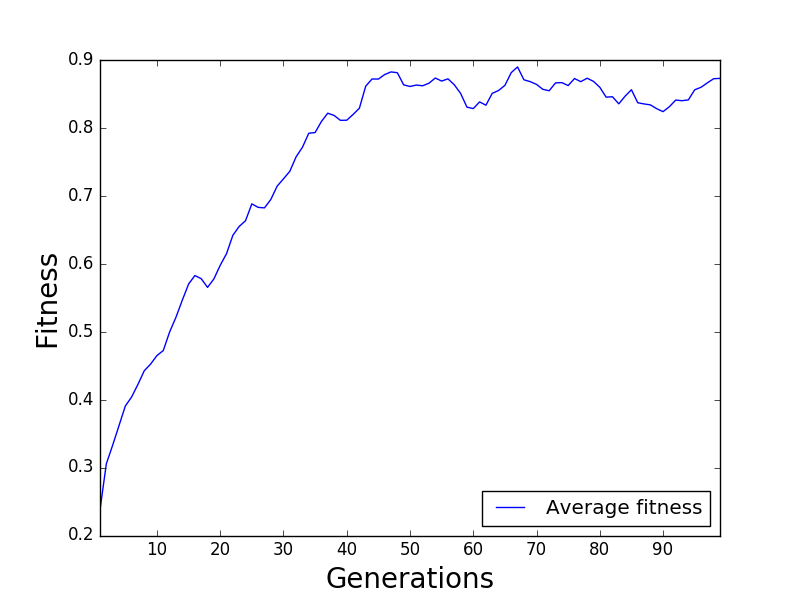
\includegraphics[width=0.49\linewidth]{fig/Results/Exp1/Fitness1}\label{fig:Fitness1}}
    \hfill
    \subfigure[]{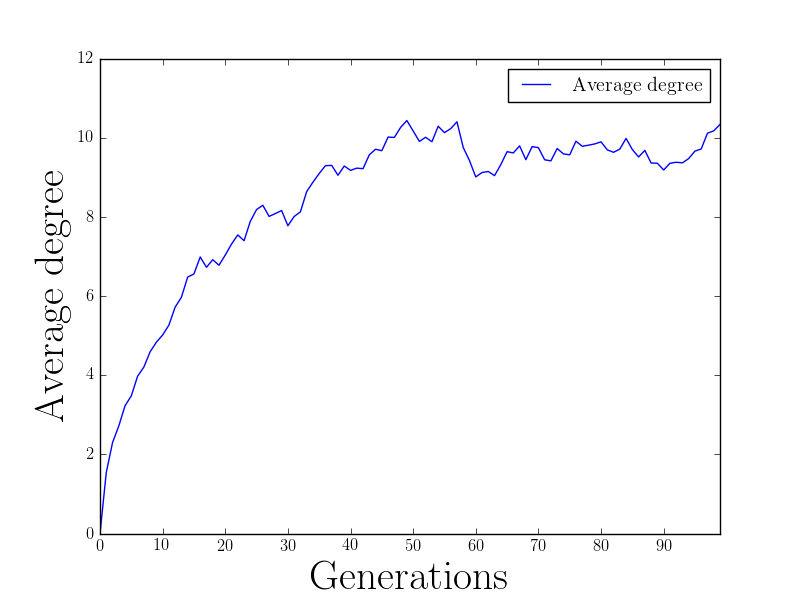
\includegraphics[width=0.49\linewidth]{fig/Results/Exp1/Degree1}\label{fig:Degree1}}
    \caption{Results from experiment 1. \subref{fig:Fitness1}: the average fitness and \subref{fig:Degree1}: the average degree.}
    \label{fig:exp1.0}
\end{figure}
\begin{figure}
    \centering
    \ContinuedFloat
    \subfigure[]{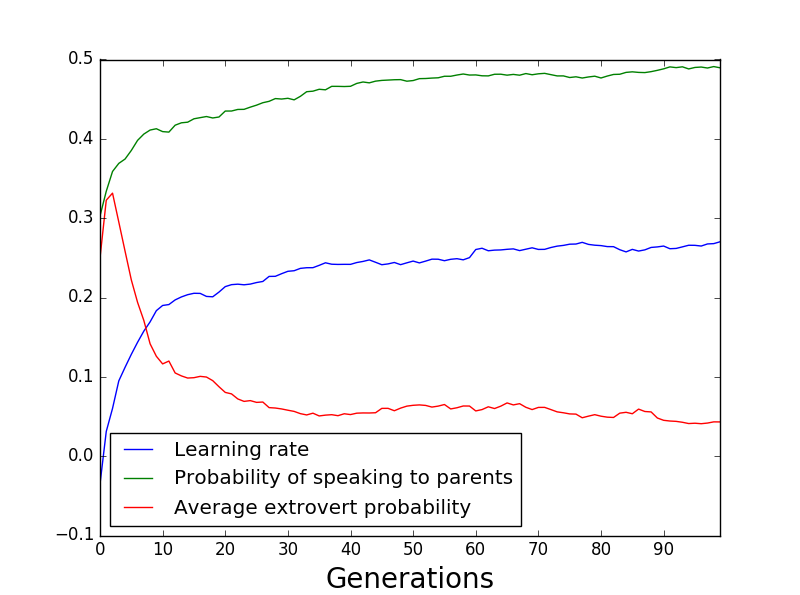
\includegraphics[width=0.49\linewidth]{fig/Results/Exp1/Genes1}\label{fig:Genes1}}
    \hfill
    \subfigure[]{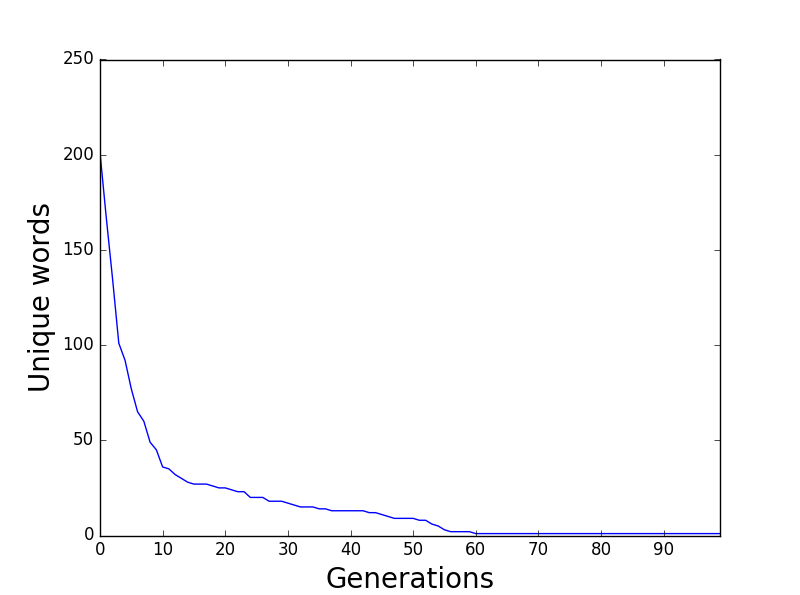
\includegraphics[width=0.49\linewidth]{fig/Results/Exp1/UniqueWords1}\label{fig:uniqueWords1}}
    \par \bigskip
    \subfigure[]{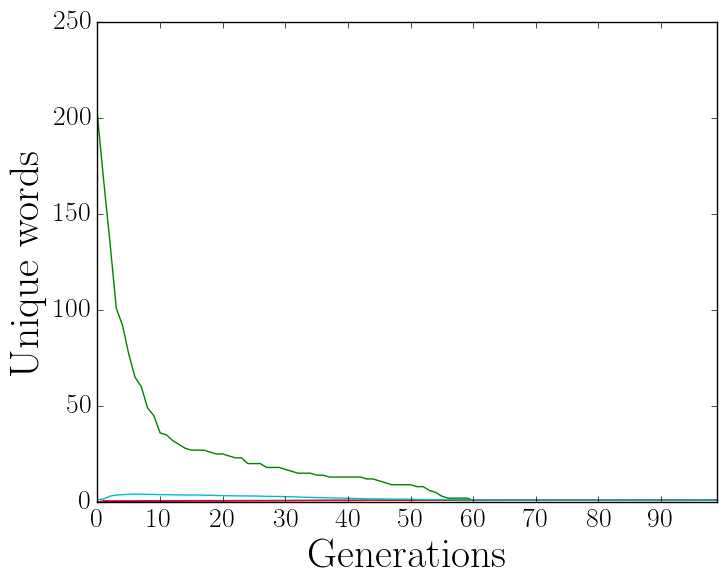
\includegraphics[width=0.49\linewidth]{fig/Results/Exp1/Vocabulary1}\label{fig:Vocabulary1}}
    \hfill
    \subfigure[]{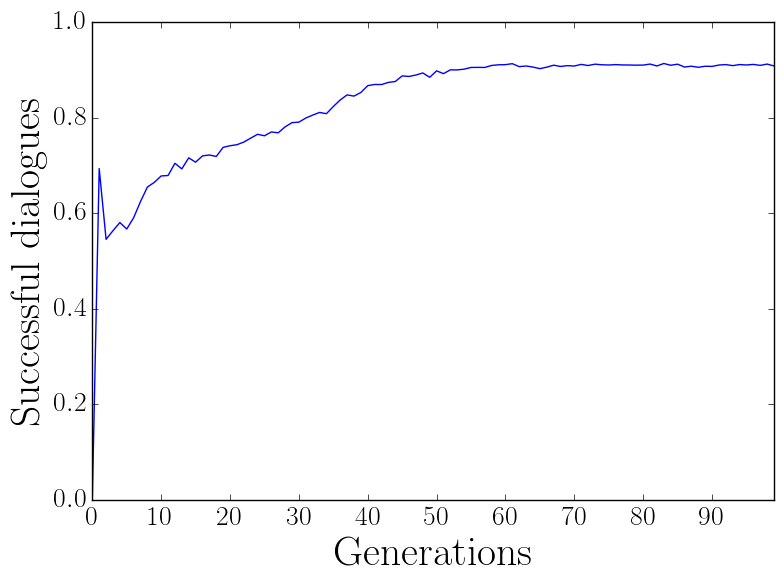
\includegraphics[width=0.49\linewidth]{fig/Results/Exp1/SuccDialogues1}\label{fig:succDia1}}
    \caption{Results from experiment 1. \subref{fig:Genes1}: the evolution of the traits from the genome. The three graphs in the figure are the green graph which is the average probability of conducting parent-child dialogues, the blue graph which is the average learning rate, and the  red graph which is the average probability of acting extrovertly. \subref{fig:uniqueWords1}: the number of unique highest ranked words in the population. \subref{fig:Vocabulary1}: the average vocabulary size. \subref{fig:succDia1}: successful dialogues divided by total number of dialogues.}
    \label{fig:exp1.1}
\end{figure}
\begin{figure}[htbp]
    \centering
    \subfigure[]{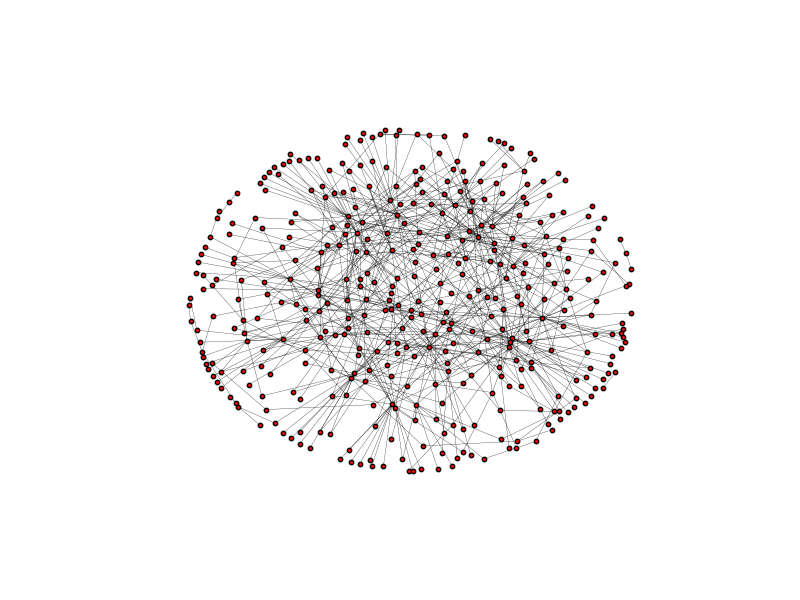
\includegraphics[width=0.49\linewidth]{fig/Results/Exp1/_graph5}\label{fig:exp1SN5}}
    \hfill
    \subfigure[]{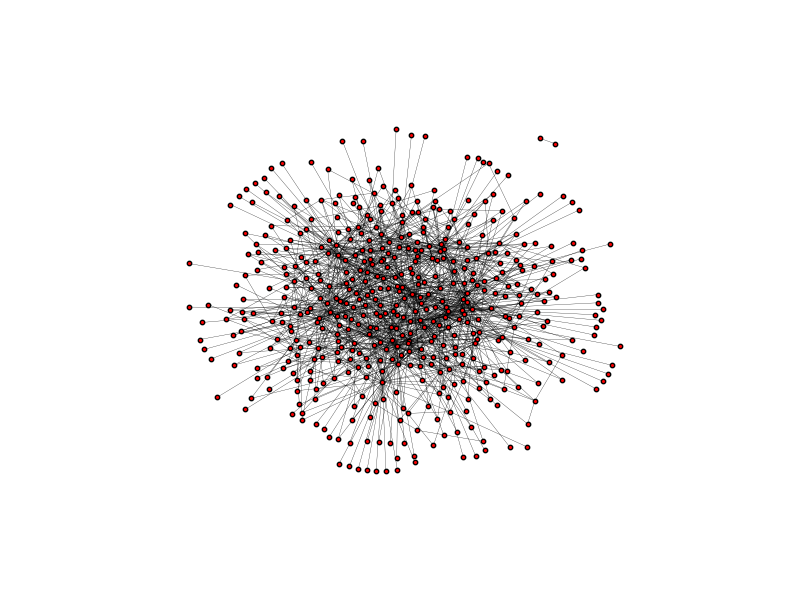
\includegraphics[width=0.49\linewidth]{fig/Results/Exp1/_graph20}\label{fig:exp1SN20}}
    \par \bigskip
    \subfigure[]{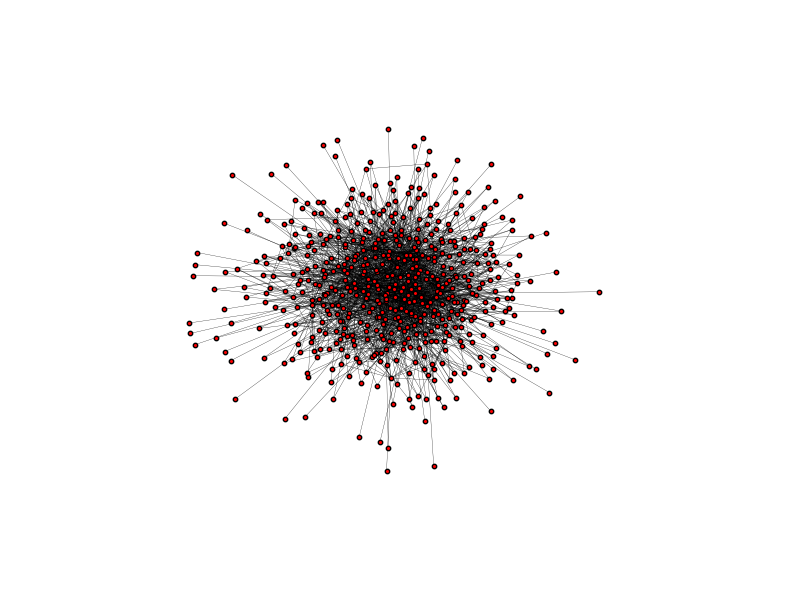
\includegraphics[width=0.49\linewidth]{fig/Results/Exp1/_graph40}\label{fig:exp1SN40}}
    \hfill
    \subfigure[]{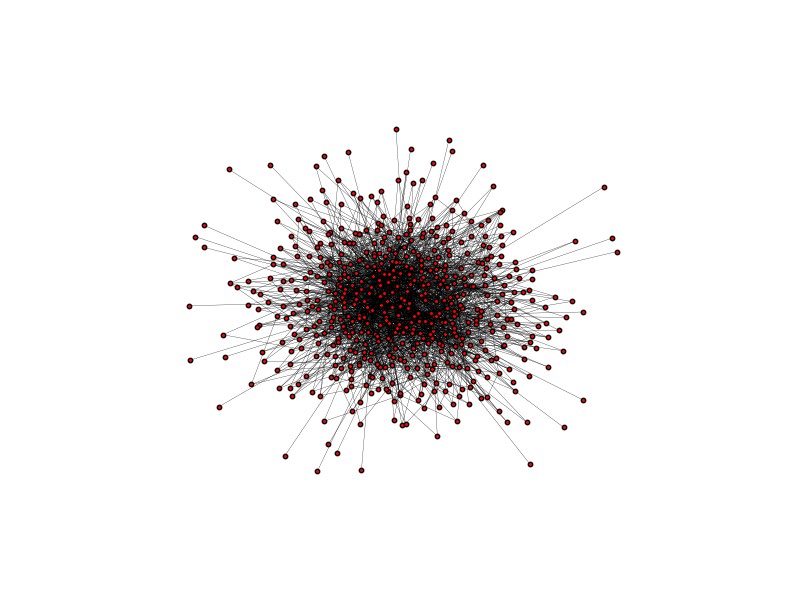
\includegraphics[width=0.49\linewidth]{fig/Results/Exp1/_graph100}\label{fig:exp1SN100}}
    \caption{Snapshots of the social network of experiment 1 at generation 5\subref{fig:exp1SN5}, 20\subref{fig:exp1SN20}, 40\subref{fig:exp1SN40}, and 100\subref{fig:exp1SN100}.}
    \label{fig:exp1.2}
\end{figure}

\clearpage
\subsection{Experiment 2 - Small population}
This experiment was conducted with a population of 100. See Figures~\ref{fig:exp2.0}, \ref{fig:exp2.1}, and \ref{fig:exp2.2} for the Figures related to this experiment. The variance seems to be higher with fewer agents, causing the average fitness and degree to vary more from one generation to another, as seen in Figures~\ref{fig:exp2.0}\subref{fig:Fitness2} and \ref{fig:exp2.0}\subref{fig:Degree2}. The average fitness seems to stabilise at about $0.85$ after generation $30$, which was earlier than in the main experiment. The percentage of successful dialogues reached $90\%$ after only $15$ generations, as seen in Figure~\ref{fig:exp2.1}\subref{fig:succDia2}, and the number of unique highest weighted words reached $1$ after $15$ generations as well, as seen in Figure~\ref{fig:exp2.1}\subref{fig:uniqueWords2}. At generation $5$, the social network consisted of a few agents with two or three edges per agent, as seen in Figure~\ref{fig:exp2.2}\subref{fig:exp2SN5}. Up until generation $40$, the social network became more and more dense for each generation that went by, as seen in Figure~\ref{fig:exp2.2}\subref{fig:exp2SN40}. Between generation $40$ and $100$, there seemed to be little change in the structure of the social network, as seen in Figure~\ref{fig:exp2.2}\subref{fig:exp2SN100}.

\begin{figure}[htbp]
    \centering
    \subfigure[]{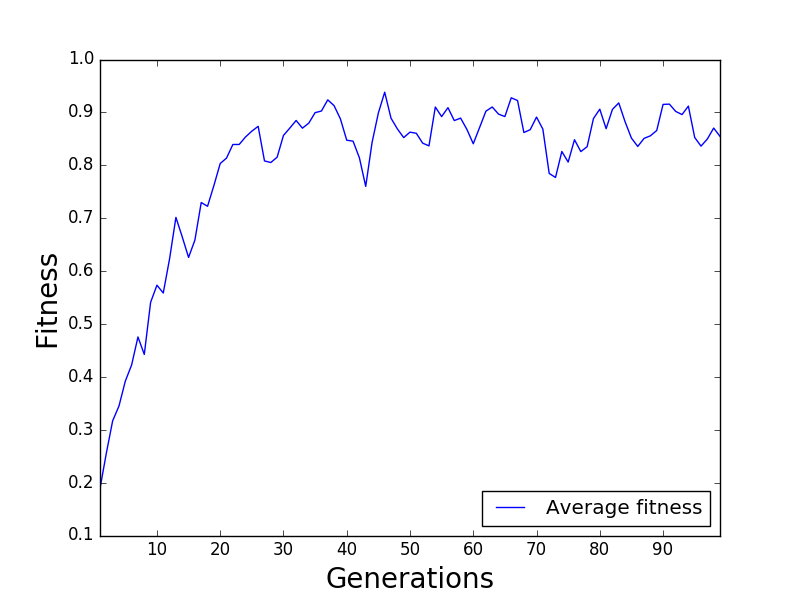
\includegraphics[width=0.49\linewidth]{fig/Results/Exp2/Fitness1}\label{fig:Fitness2}}
    \hfill
    \subfigure[]{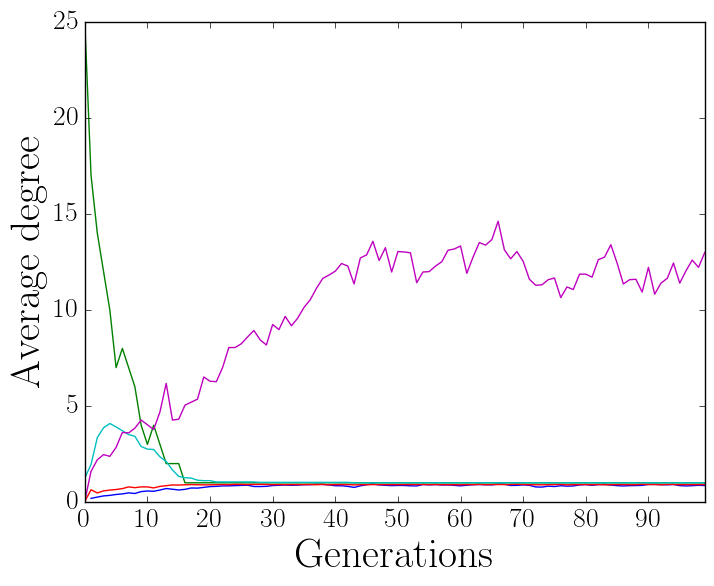
\includegraphics[width=0.49\linewidth]{fig/Results/Exp2/Degree1}\label{fig:Degree2}}
    \caption{Results from experiment 2. \subref{fig:Fitness2}: the average fitness and \subref{fig:Degree2}: the average degree.}
    \label{fig:exp2.0}
\end{figure}
\begin{figure}
    \centering
    \ContinuedFloat
    \subfigure[]{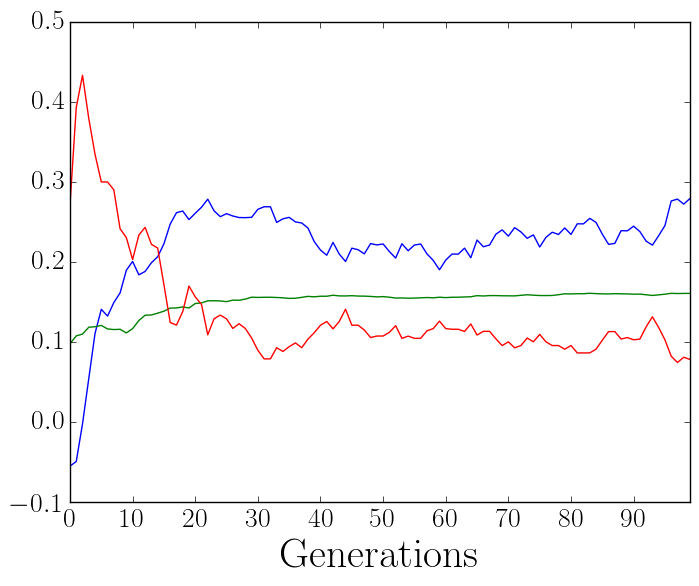
\includegraphics[width=0.49\linewidth]{fig/Results/Exp2/Genes1}\label{fig:exp2Genes}}
    \hfill
    \subfigure[]{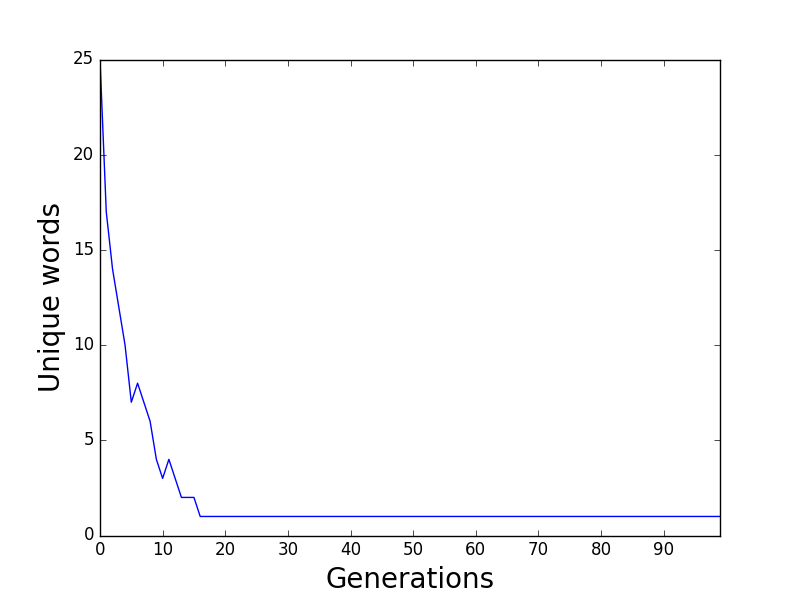
\includegraphics[width=0.49\linewidth]{fig/Results/Exp2/UniqueWords1}\label{fig:uniqueWords2}}
    \par \bigskip
    \subfigure[]{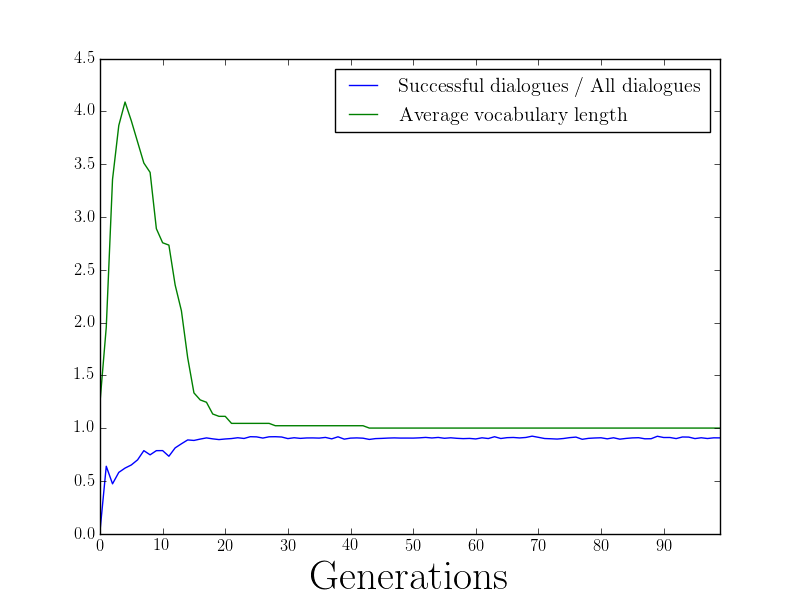
\includegraphics[width=0.49\linewidth]{fig/Results/Exp2/Vocabulary1}\label{fig:Vocabulary2}}
    \hfill
    \subfigure[]{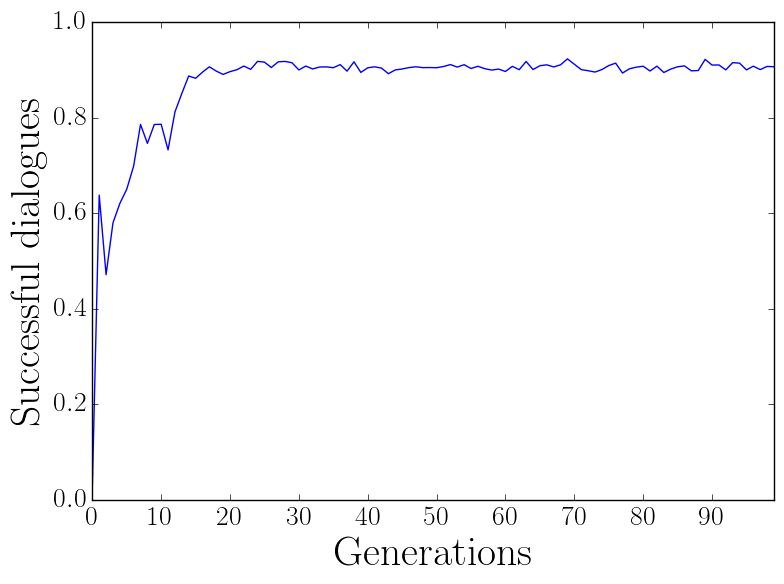
\includegraphics[width=0.49\linewidth]{fig/Results/Exp2/SuccDialogues1}\label{fig:succDia2}}
    \caption{Results from experiment 2. \subref{fig:exp2Genes}: the evolution of the traits from the genome. The three graphs in the figure are the green graph which is the average probability of conducting parent-child dialogues, the blue graph which is the average learning rate, and the  red graph which is the average probability of acting extrovertly. \subref{fig:uniqueWords2}: the number of unique highest ranked words in the population. \subref{fig:Vocabulary2}: average vocabulary size. \subref{fig:succDia2}: successful dialogues divided by total number of dialogues.}
    \label{fig:exp2.1}
\end{figure}
\begin{figure}[htbp]
    \centering
    \subfigure[]{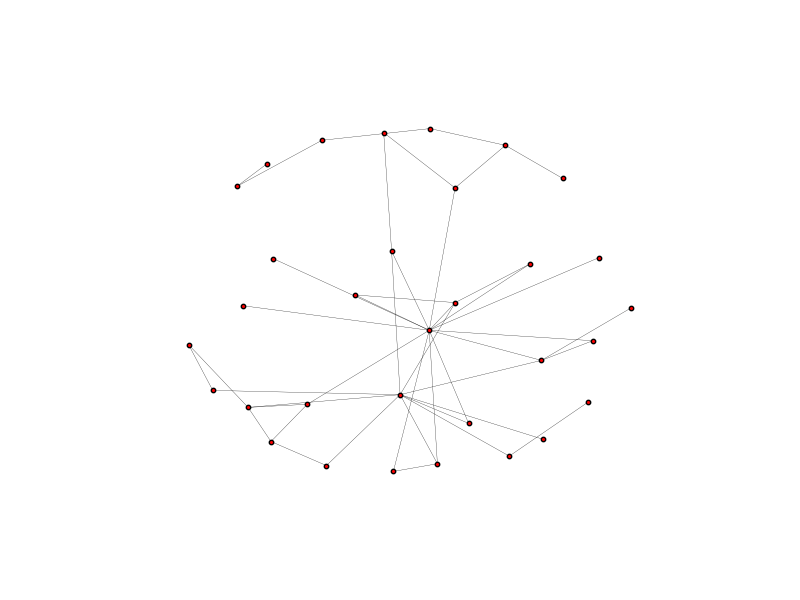
\includegraphics[width=0.49\linewidth]{fig/Results/Exp2/_graph5}\label{fig:exp2SN5}}
    \hfill
    \subfigure[]{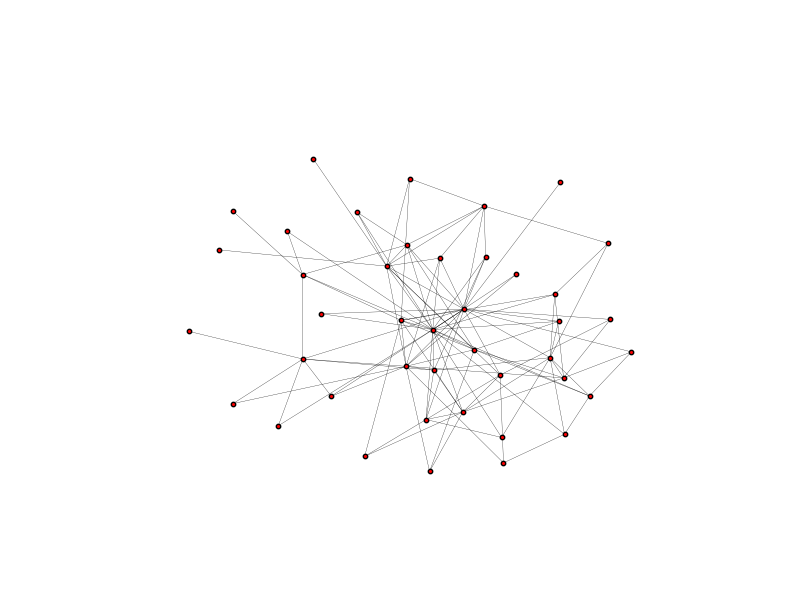
\includegraphics[width=0.49\linewidth]{fig/Results/Exp2/_graph20}\label{fig:exp2SN20}}
    \subfigure[]{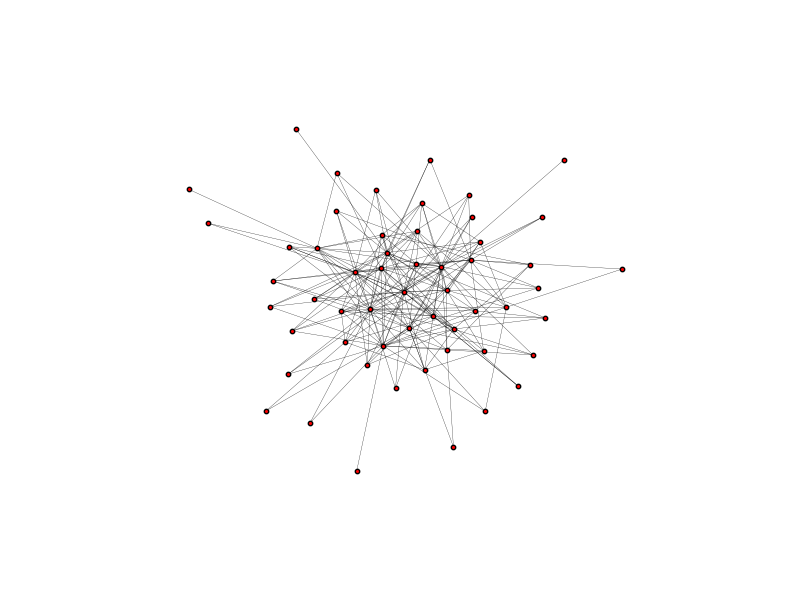
\includegraphics[width=0.49\linewidth]{fig/Results/Exp2/_graph40}\label{fig:exp2SN40}}
    \hfill
    \subfigure[]{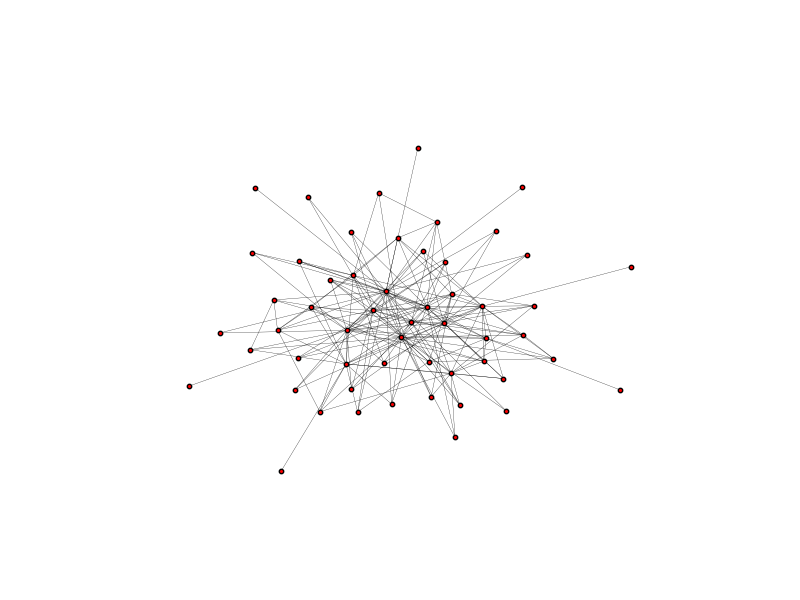
\includegraphics[width=0.49\linewidth]{fig/Results/Exp2/_graph100}\label{fig:exp2SN100}}
    \caption{Snapshots of the social network of experiment 2 at generation 5\subref{fig:exp2SN5}, 20\subref{fig:exp2SN20}, 40\subref{fig:exp2SN40}, and 100\subref{fig:exp2SN100}.}
    \label{fig:exp2.2}
\end{figure}

\clearpage
\subsection{Experiment 3 - Large population}
This experiment was performed with a population of $10000$. See Figure~\ref{fig:exp3.0}, \ref{fig:exp3.0} for the figures related to this experiment. The results show that when there were many agents, they required more time to reach consensus, as seen in Figure~\ref{fig:exp3.1}\subref{fig:uniqueWords3}. In fact, after 100 generations, the agents had not reached an agreement upon one word. This lead to communication more often being unsuccessful, as seen in Figure~\ref{fig:exp3.1}\subref{fig:succDia3}, which again lead to the average fitness and degree being lower than in the results from the main experiment, as seen in Figures~\ref{fig:exp3.0}\subref{fig:Fitness3} and \ref{fig:exp3.0}\subref{fig:Degree3}. The difference in the social network is that the agents were divided into one main group and several other groups of two to three agents for the first generations, as seen in Figure~\ref{fig:exp3.2}.

\begin{figure}[htbp]
    \centering
    \subfigure[]{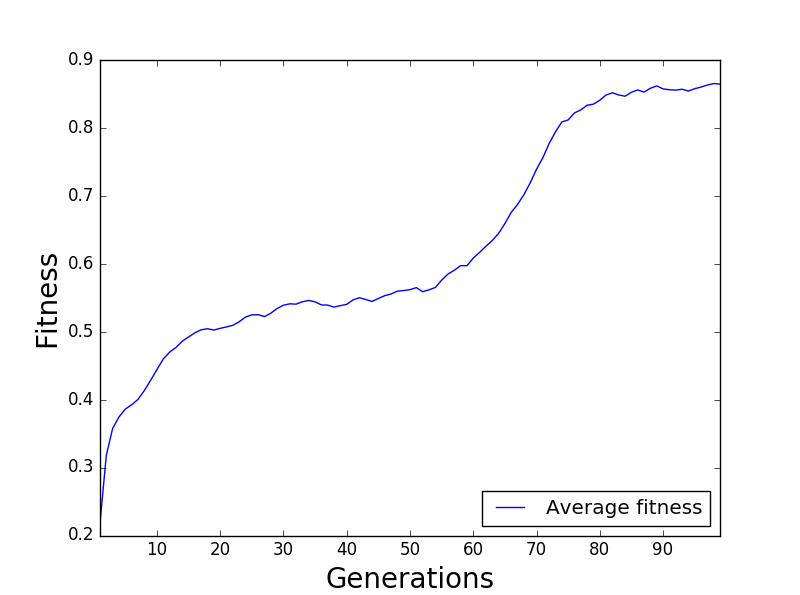
\includegraphics[width=0.49\linewidth]{fig/Results/Exp3/Fitness1}\label{fig:Fitness3}}
    \hfill
    \subfigure[]{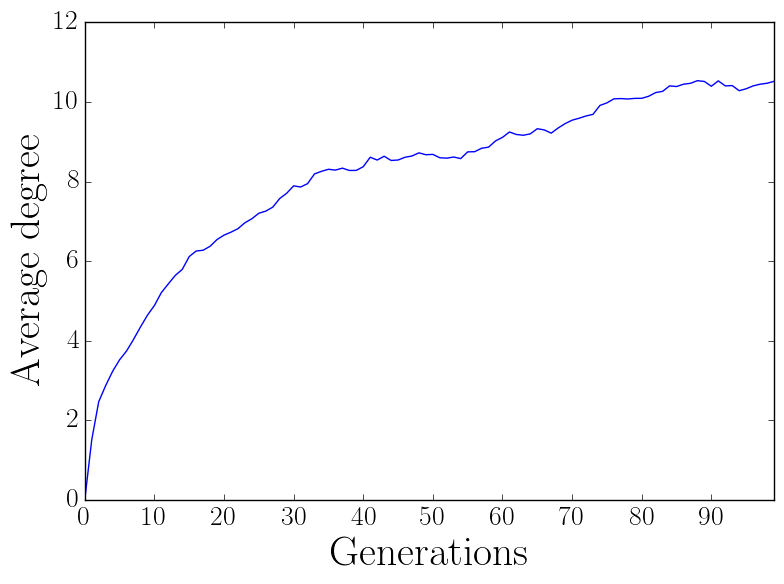
\includegraphics[width=0.49\linewidth]{fig/Results/Exp3/Deg1}\label{fig:Degree3}}
    \caption{Results from experiment 3. \subref{fig:Fitness3}: the average fitness and \subref{fig:Degree3}: the average degree.}
    \label{fig:exp3.0}
\end{figure}
\begin{figure}
    \centering
    \ContinuedFloat
    \subfigure[]{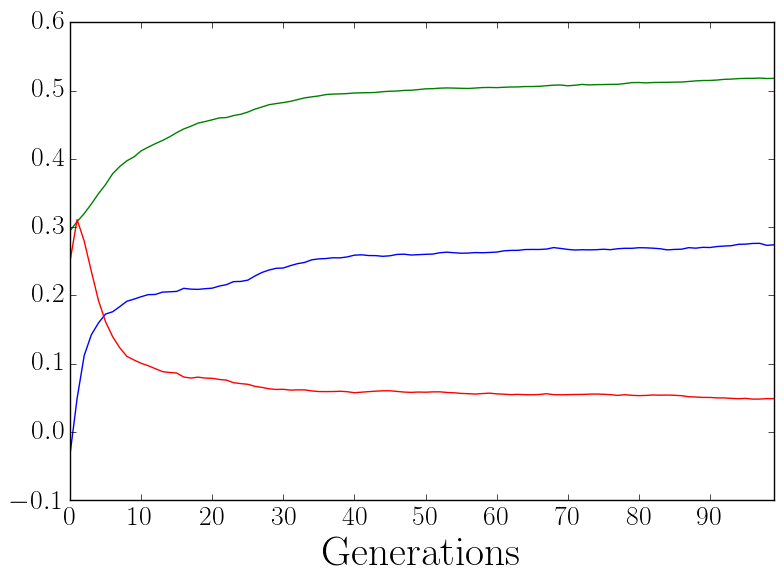
\includegraphics[width=0.49\linewidth]{fig/Results/Exp3/Genes1}\label{fig:exp3Genes}}
    \hfill
    \subfigure[]{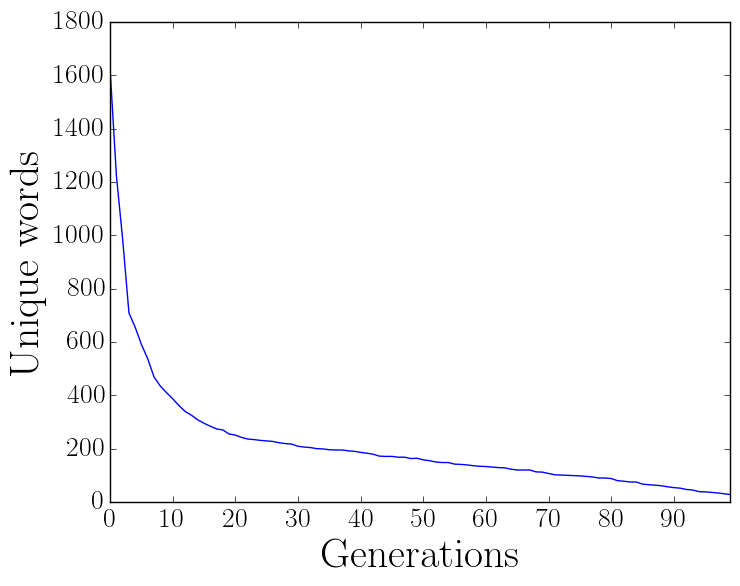
\includegraphics[width=0.49\linewidth]{fig/Results/Exp3/UniqueWords1}\label{fig:uniqueWords3}}
    \par \bigskip
    \subfigure[]{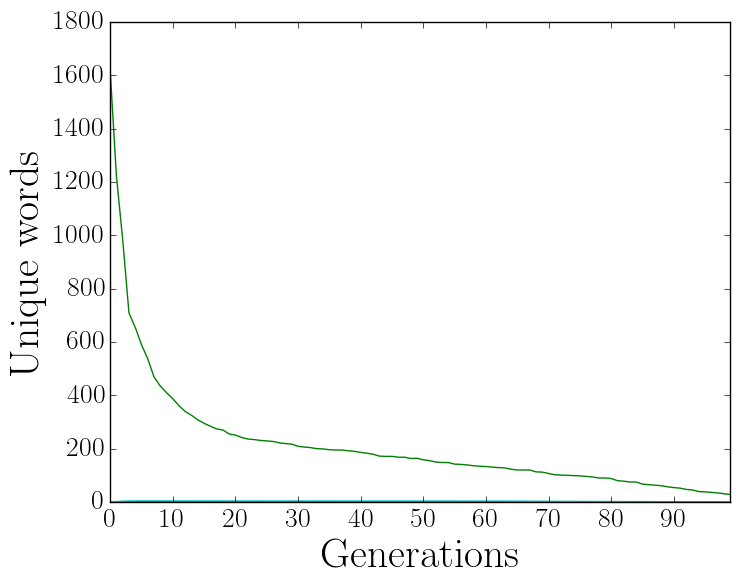
\includegraphics[width=0.49\linewidth]{fig/Results/Exp3/Vocabulary1}\label{fig:Vocabulary3}}
    \hfill
    \subfigure[]{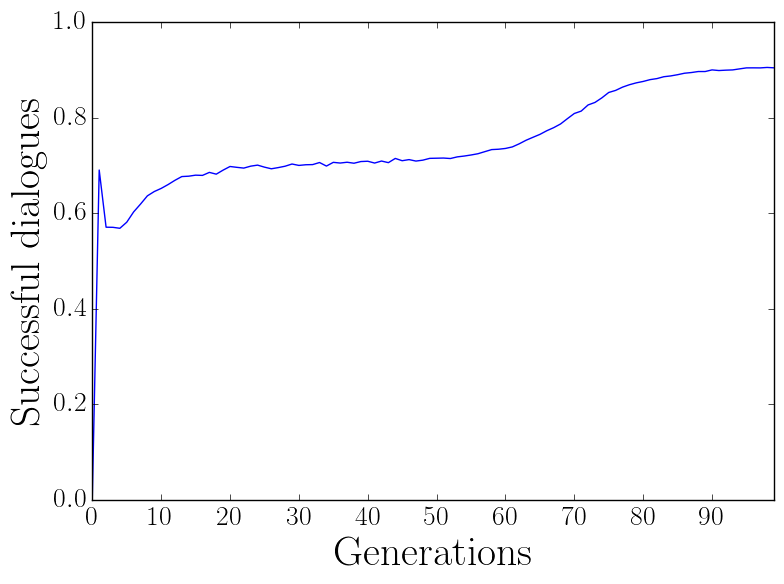
\includegraphics[width=0.49\linewidth]{fig/Results/Exp3/SuccDialogues1}\label{fig:succDia3}}
    \caption{Results from experiment 3. \subref{fig:exp3Genes}: the evolution of the traits from the genome. The three graphs in the figure are the green graph which is the average probability of conducting parent-child dialogues, the blue graph which is the average learning rate, and the  red graph which is the average probability of acting extrovertly. \subref{fig:uniqueWords3}: the number of unique highest ranked words in the population. \subref{fig:Vocabulary3}: average vocabulary size. \subref{fig:succDia3}: successful dialogues divided by total number of dialogues.}
    \label{fig:exp3.1}
\end{figure}
\begin{figure}[htbp]
    \centering
    \subfigure[]{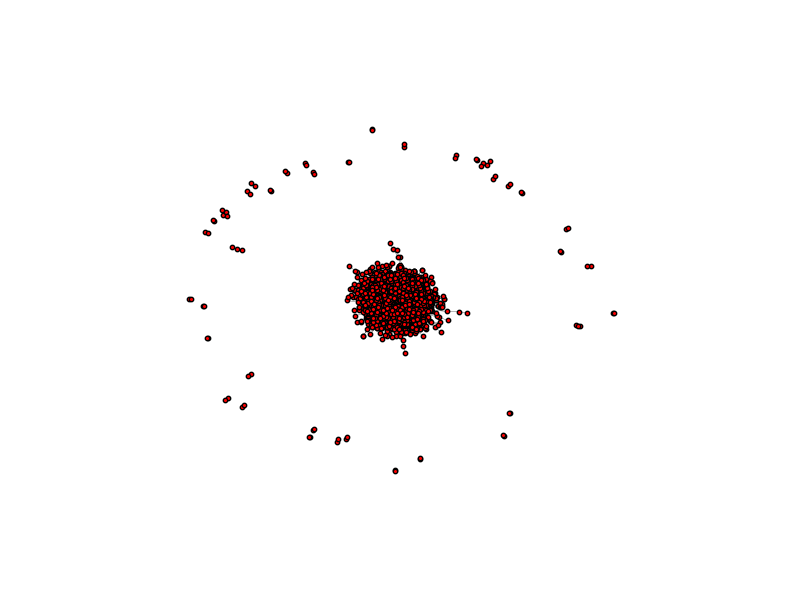
\includegraphics[width=0.49\linewidth]{fig/Results/Exp3/_graph5}\label{fig:exp3SN5}}
    \hfill
    \subfigure[]{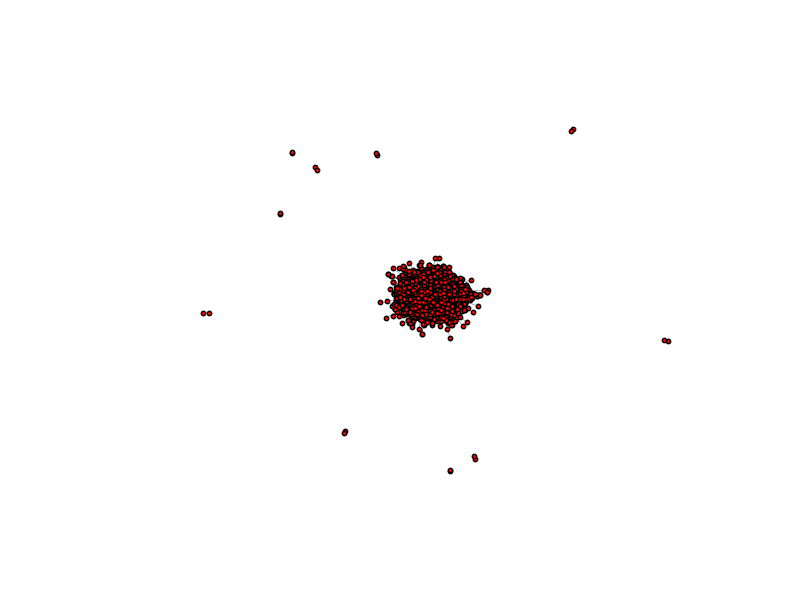
\includegraphics[width=0.49\linewidth]{fig/Results/Exp3/_graph10}\label{fig:exp3SN10}}
    \par \bigskip
    \subfigure[]{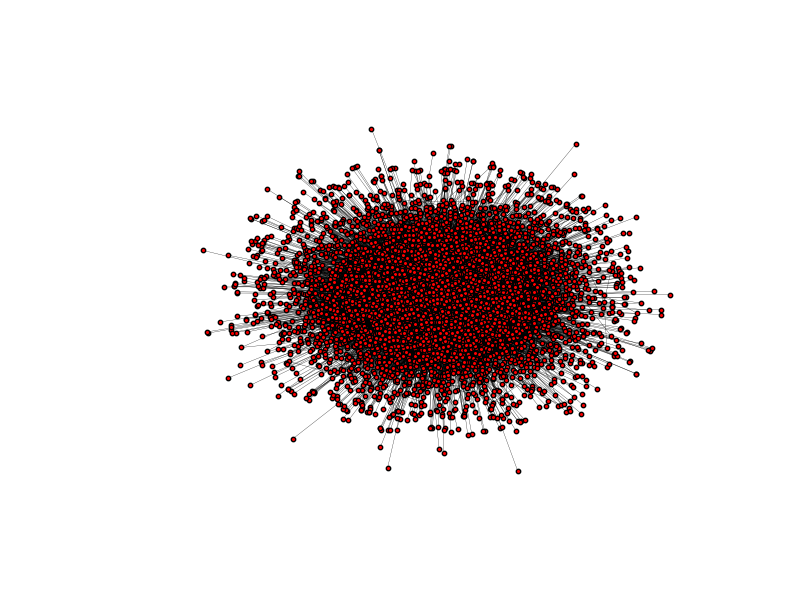
\includegraphics[width=0.49\linewidth]{fig/Results/Exp3/_graph40}\label{fig:exp3SN40}}
    \hfill
    \subfigure[]{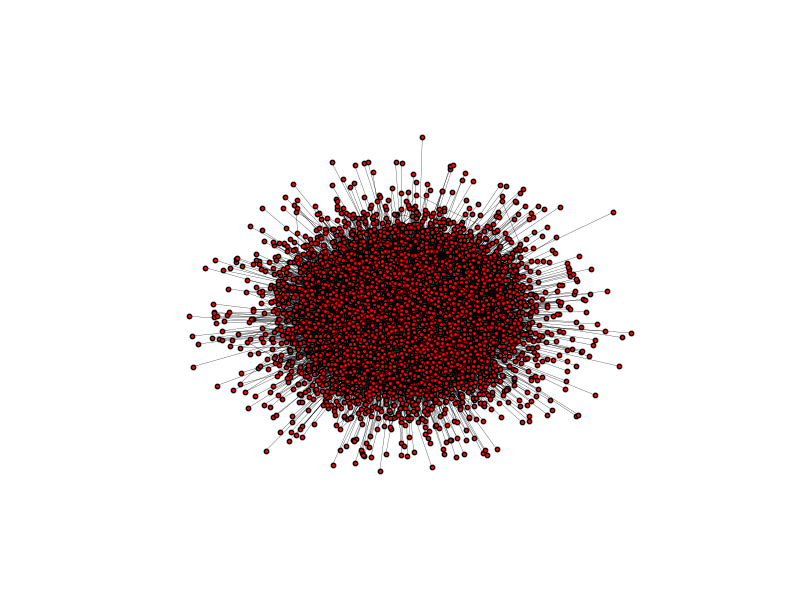
\includegraphics[width=0.49\linewidth]{fig/Results/Exp3/_graph100}\label{fig:exp3SN100}}
    \caption{Snapshots of the social network of experiment 3 at generation 5\subref{fig:exp3SN5}, 10\subref{fig:exp3SN10}, 40\subref{fig:exp3SN40}, and 100\subref{fig:exp3SN100}.}
    \label{fig:exp3.2}
\end{figure}

\clearpage
\subsection{Experiment 4 - Dialogues}
This experiment was conducted with $d = 5$, meaning that each generation conducted five times as many dialogues as in experiment $1$. See Figures~\ref{fig:exp4.0} and \ref{fig:exp4.1} for the graphs related to this experiment. The average degree increased when five times as many dialogues were conducted, as seen in Figure~\ref{fig:exp4.0}\subref{fig:Degree4}. The increase in dialogues ensures that each agent has more and stronger connections leading to a higher average fitness, as seen in Figure~\ref{fig:exp4.0}\subref{fig:Fitness4}. The simulation reached consensus at about the same time as the main experiment, as seen in Figure~\ref{fig:exp4.1}\subref{fig:uniqueWords4}. The probability of acting extrovertly stagnated at about $16\%$, which is almost three times more than experiment 1, as seen in Figure~\ref{fig:exp4.1}\subref{fig:Genes4} The social network evolved similarly as in the main experiment, except that the agents on average had more edges.

\begin{figure}[htbp]
    \centering
    \subfigure[]{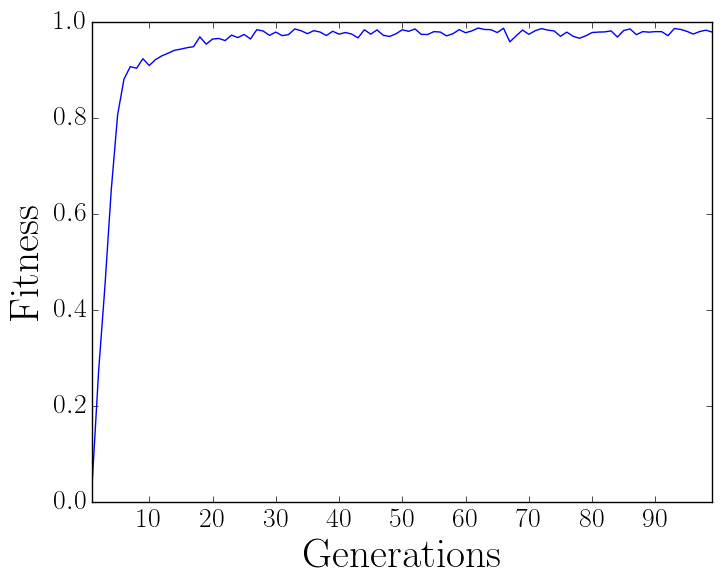
\includegraphics[width=0.49\linewidth]{fig/Results/Exp4/Fitness1}\label{fig:Fitness4}}
    \hfill
    \subfigure[]{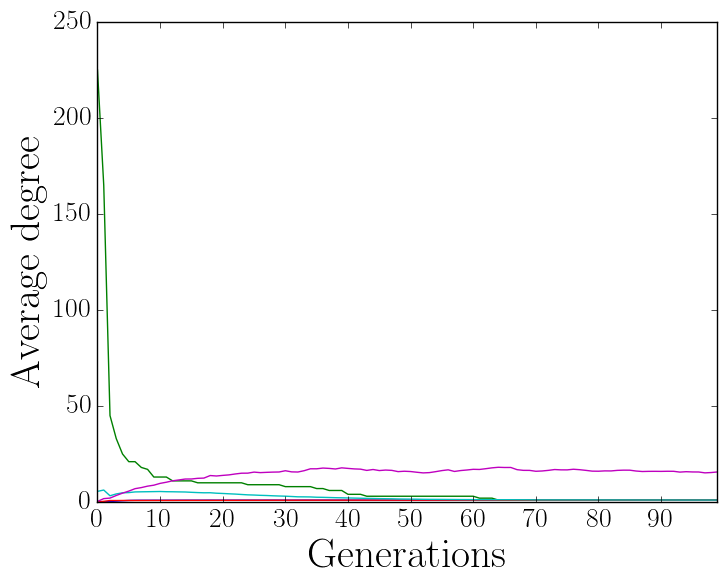
\includegraphics[width=0.49\linewidth]{fig/Results/Exp4/Degree1}\label{fig:Degree4}}
    \caption{Results from experiment 4. \subref{fig:Fitness4}: the average fitness and \subref{fig:Degree4}: the average degree.}
    \label{fig:exp4.0}
\end{figure}
\begin{figure}
    \centering
    \ContinuedFloat
    \subfigure[]{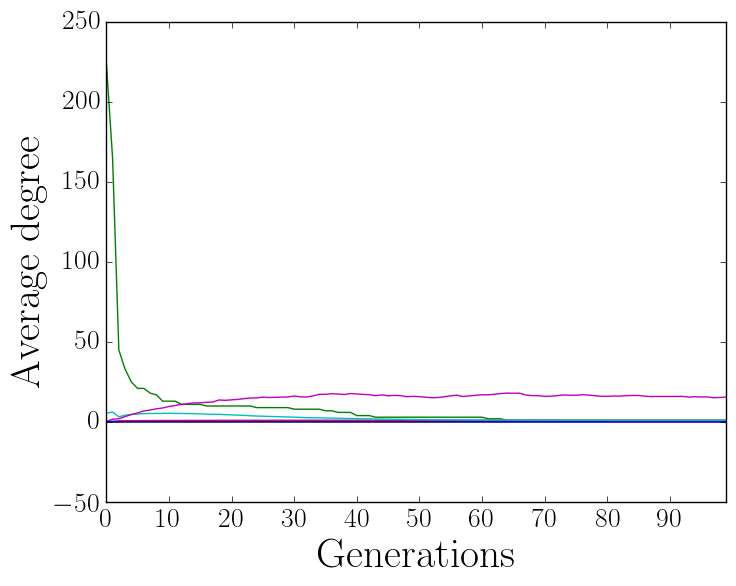
\includegraphics[width=0.49\linewidth]{fig/Results/Exp4/genes1}\label{fig:Genes4}}
    \hfill
    \subfigure[]{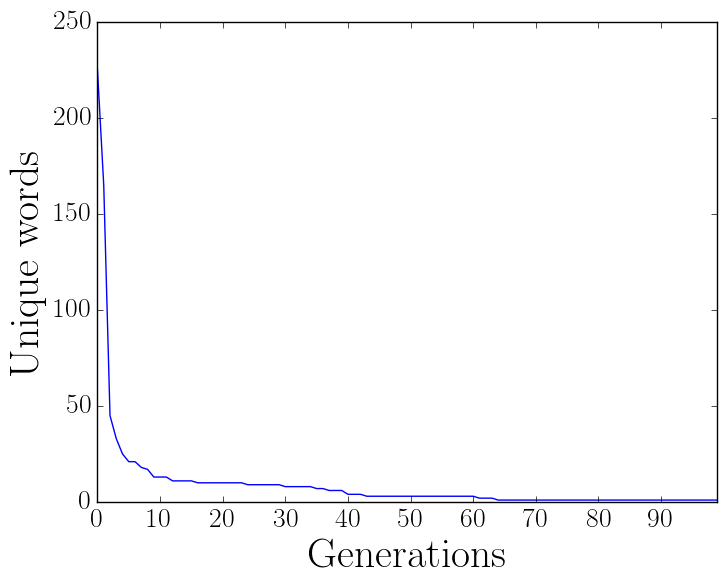
\includegraphics[width=0.49\linewidth]{fig/Results/Exp4/UniqueWords1}\label{fig:uniqueWords4}}
    \par \bigskip
    \subfigure[]{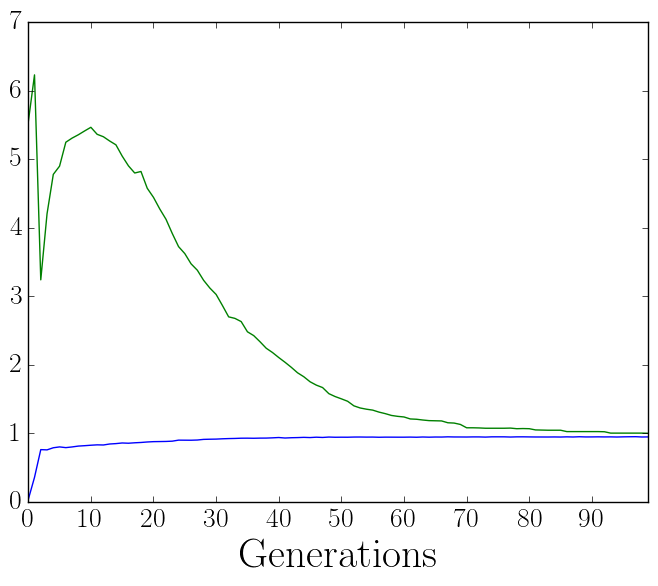
\includegraphics[width=0.49\linewidth]{fig/Results/Exp4/Vocabulary1}\label{fig:Vocabulary4}}
    \hfill
    \subfigure[]{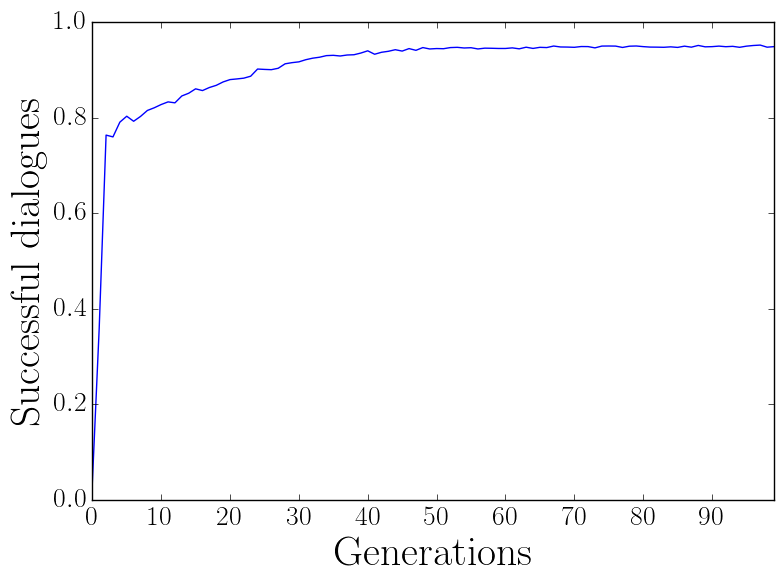
\includegraphics[width=0.49\linewidth]{fig/Results/Exp4/SuccDialogues1}\label{fig:succDia4}}
    \caption{Results from experiment 4. \subref{fig:Genes4}: the evolution of the traits from the genome. The three graphs in the figure are the green graph which is the average probability of conducting parent-child dialogues, the blue graph which is the average learning rate, and the  red graph which is the average probability of acting extrovertly. \subref{fig:uniqueWords4}: the number of unique highest ranked words in the population. \subref{fig:Vocabulary4}: average vocabulary size. \subref{fig:succDia4}: successful dialogues divided by total number of dialogues.}
    \label{fig:exp4.1}
\end{figure}

\clearpage
\subsection{Experiment 5 - Less Parent-child dialogues}
This experiment was conducted with the constant $\delta = 1$. $\delta$ is related to the probability of a child having its first dialogues with its parents. See figures~\ref{fig:exp5.0} and \ref{fig:exp5.1} for the figures related to this experiment. The simulation was ran for $150$ generations, e.g. $g = 150$, because it did not reach consensus after $100$ generations, and knowing how this simulation evolved up until consensus might be interesting. The average fitness increased slowly during the entire simulation, as seen in Figure~\ref{fig:exp5.0}\subref{fig:Fitness5}. The average degree reached four at generation $70$, and during the next $80$ generations the average only increased by $0.5$, as seen in Figure~\ref{fig:exp5.0}\subref{fig:Degree5}. The percentage of successful dialogues quickly reached $60\%$, and slowly increased during the entire simulation ending at $93\%$, as seen in Figure~\ref{fig:exp5.1}\subref{fig:succDia5}. The average vocabulary size increased during the first $25$ generations, and then decreased and ended at $1.04$, as seen in Figure~\ref{fig:exp5.1}\subref{fig:Vocabulary5}. The simulation reached consensus at generation $127$, as seen in Figure~\ref{fig:exp5.1}\subref{fig:uniqueWords5}.

\begin{figure}[htbp]
    \centering
    \subfigure[]{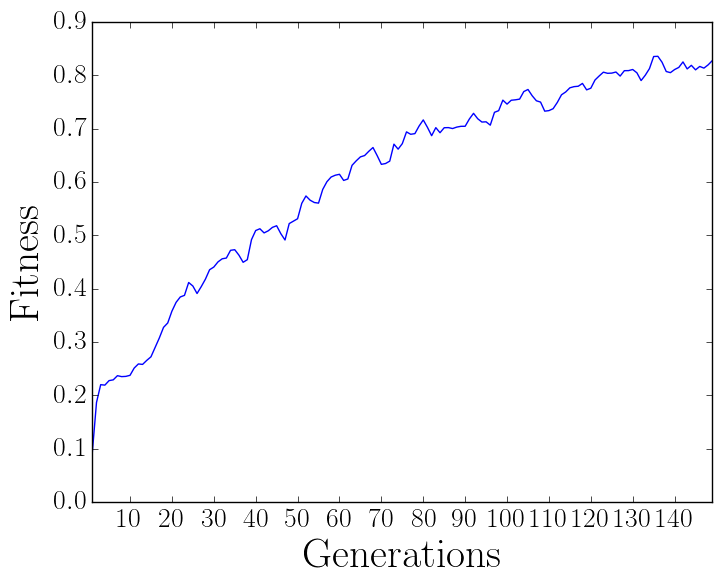
\includegraphics[width=0.49\linewidth]{fig/Results/Exp5/Fitness1}\label{fig:Fitness5}}
    \hfill
    \subfigure[]{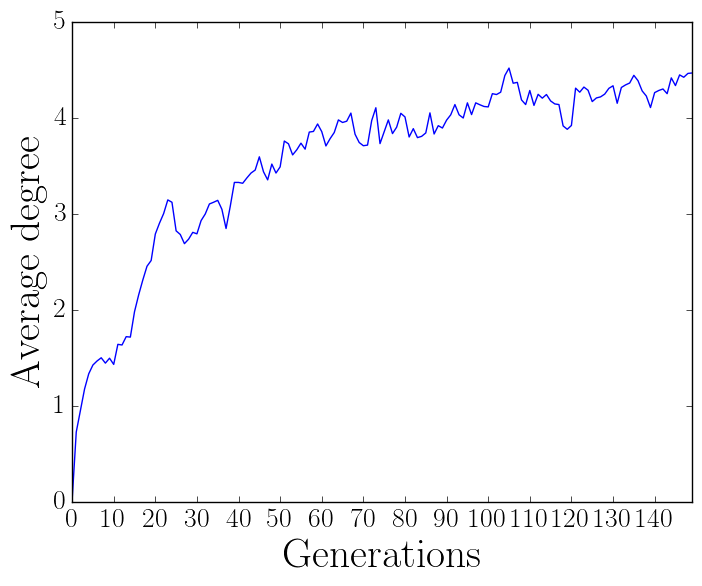
\includegraphics[width=0.49\linewidth]{fig/Results/Exp5/Degree1}\label{fig:Degree5}}
    \caption{Results from experiment 5. \subref{fig:Fitness5}: the average fitness and \subref{fig:Degree5}: the average degree.}
    \label{fig:exp5.0}
\end{figure}
\begin{figure}
    \centering
    \ContinuedFloat
    \subfigure[]{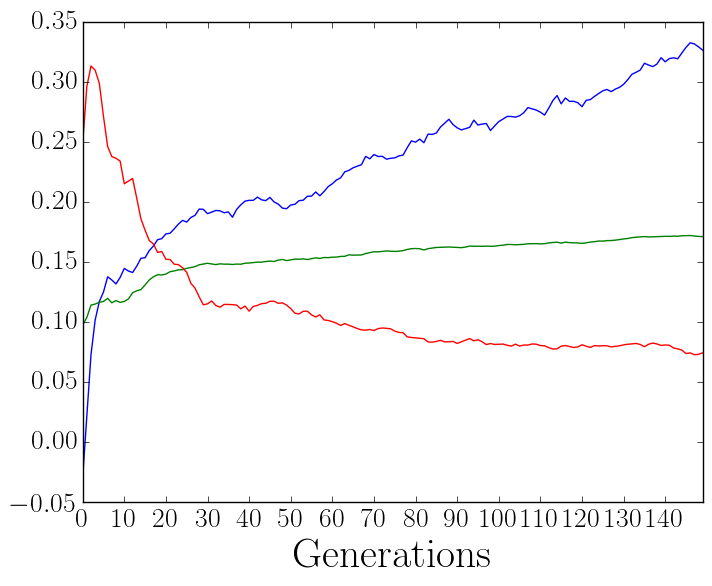
\includegraphics[width=0.49\linewidth]{fig/Results/Exp5/Genes1}\label{fig:Genes5}}
    \hfill
    \subfigure[]{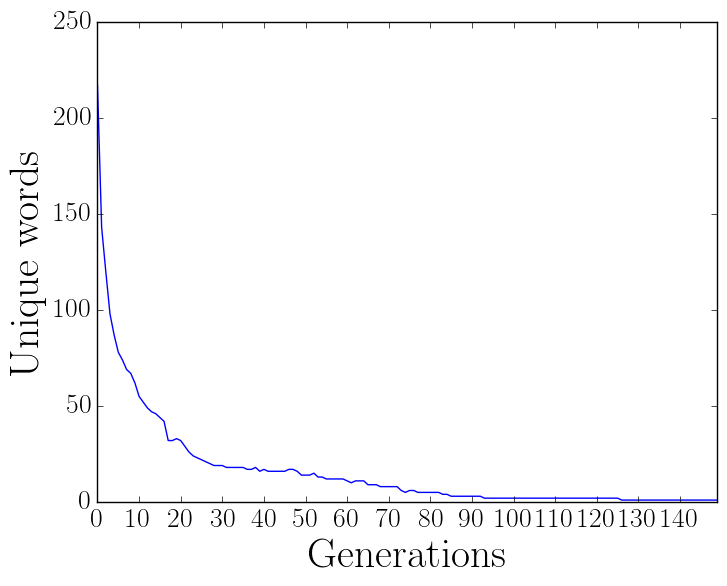
\includegraphics[width=0.49\linewidth]{fig/Results/Exp5/UniqueWords1}\label{fig:uniqueWords5}}
    \par \bigskip
    \subfigure[]{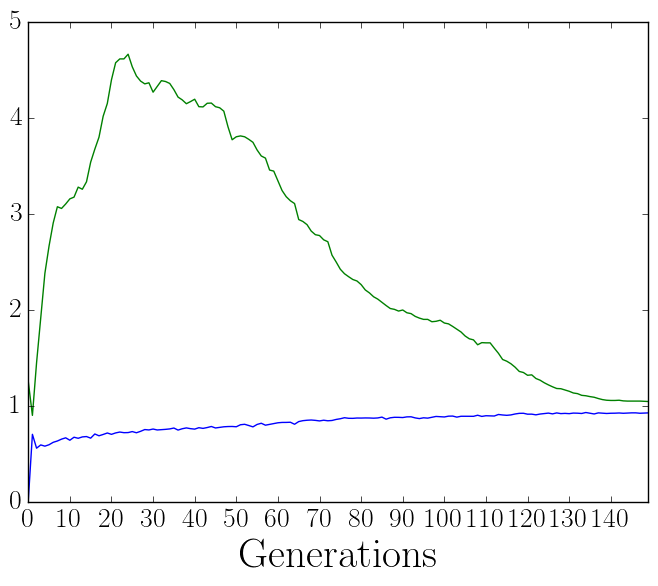
\includegraphics[width=0.49\linewidth]{fig/Results/Exp5/Vocabulary1}\label{fig:Vocabulary5}}
    \hfill
    \subfigure[]{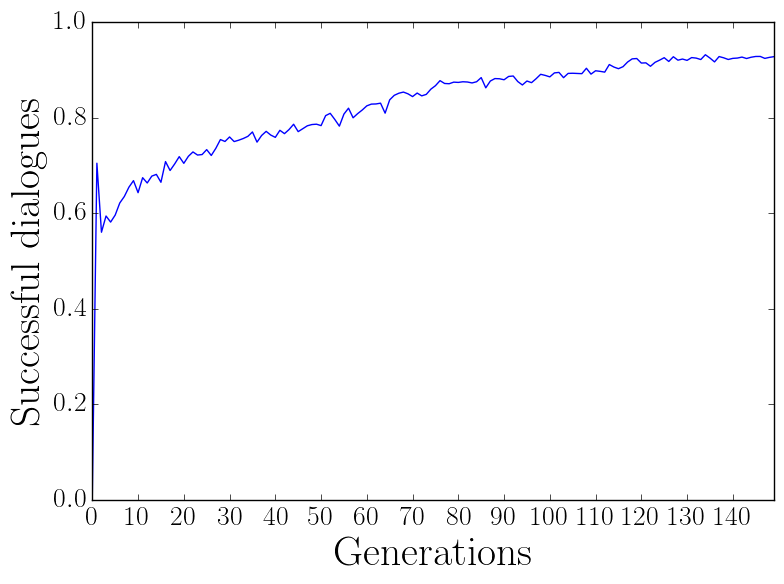
\includegraphics[width=0.49\linewidth]{fig/Results/Exp5/SuccDialogues1}\label{fig:succDia5}}
    \caption{Results from experiment 5. \subref{fig:Genes5}: the evolution of the traits from the genome. The three graphs in the figure are the green graph which is the average probability of conducting parent-child dialogues, the blue graph which is the average learning rate, and the  red graph which is the average probability of acting extrovertly. \subref{fig:uniqueWords5}: the number of unique highest ranked words in the population. \subref{fig:Vocabulary5}: average vocabulary size. \subref{fig:succDia5}: successful dialogues divided by total number of dialogues.}
    \label{fig:exp5.1}
\end{figure}

\clearpage
\subsection{Experiment 6 - Turnover}
%
Experiment 6 was performed in two parts, part 6a with $k = 0.95$ and $n = 0.7$, compared to $k = 0.9$ and $n = 0.5$ in the other experiments. This means that a larger portion (n) of the population was chosen for survival and from a larger selection pool (K). Figures~\ref{fig:exp6.0} and \ref{fig:exp6.1} show the results of experiment 6. This simulation was run for $150$ generations because the population was far away from reaching consensus after $100$ generations. The figures that display the genes and the evolution of the social network have not been included because they were similar to the ones from the main experiment. Both the average fitness and degree stabilised after about $75$ generations, as can be seen in the Figures~\ref{fig:Fitness6} and \ref{fig:Degree6}. The average degree stabilised at $11$ and the average fitness at $0.88$. The number of unique words decreased a lot during the first $20$ generations, as can be seen in Figure~\ref{fig:uniqueWords6}. The simulation did not reach consensus. It reached two unique words at generation $125$, and also ended with two unique words after all $150$ generations.   

Experiment 6b was conducted with $k = 0.95$ and $n = 0.85$ which allowed a larger portion of the fittest agents to survive each generation, giving the simulation a lower selection pressure. Experiment 6b was conducted in order to see what happened when the selection pressure was lower than in experiment 6b. Figure ~\ref{fig:uniqueWords6} compares how experiment 6a and 6b evolved towards consensus. Experiment 6b was ran for $200$ generations in order for it to reach consensus. Consensus was reached at generation $178$. At generation $125$, when experiment 6a had reached two words, this simulation had six unique words. 

\begin{figure}[htbp]
    \centering
    \subfigure[]{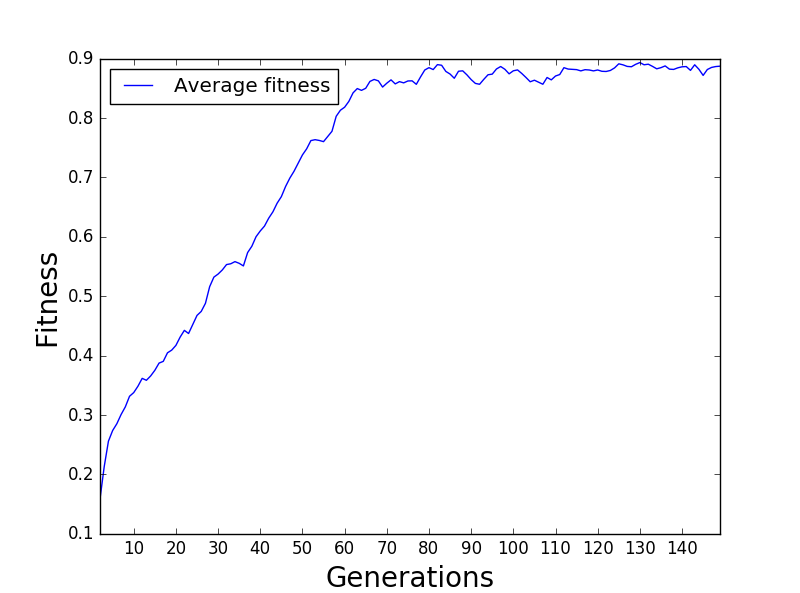
\includegraphics[width=0.49\linewidth]{fig/Results/Exp6/Fitness1}\label{fig:Fitness6}}
    \hfill
    \subfigure[]{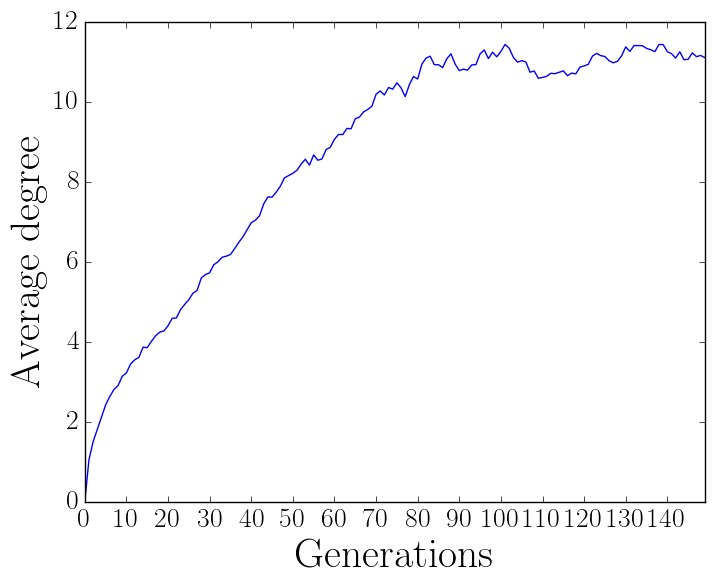
\includegraphics[width=0.49\linewidth]{fig/Results/Exp6/Degree1}\label{fig:Degree6}}
    \caption{Results from experiment 6. \subref{fig:Fitness6}: the average fitness and \subref{fig:Degree6}: the average degree.}
    \label{fig:exp6.0}
\end{figure}
\begin{figure}
    \centering
    \ContinuedFloat
    \subfigure[]{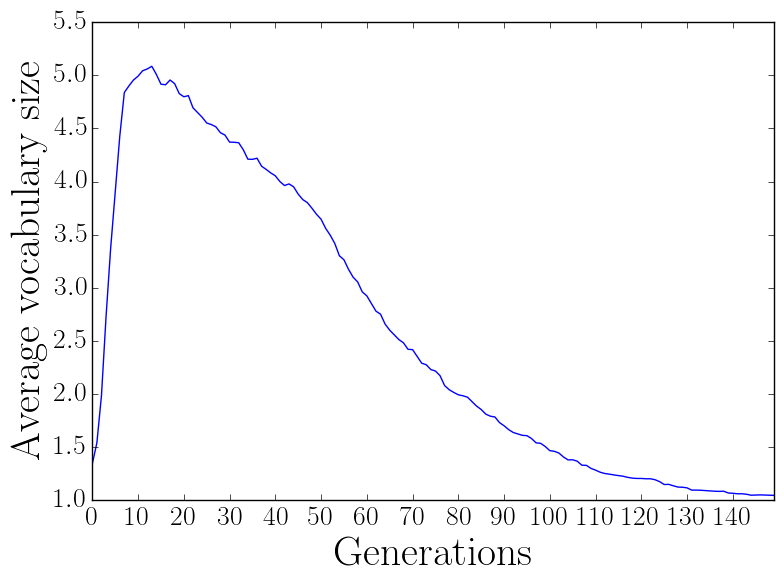
\includegraphics[width=0.49\linewidth]{fig/Results/Exp6/Vocabulary1}\label{fig:Vocabulary6}}
    \hfill
    \subfigure[]{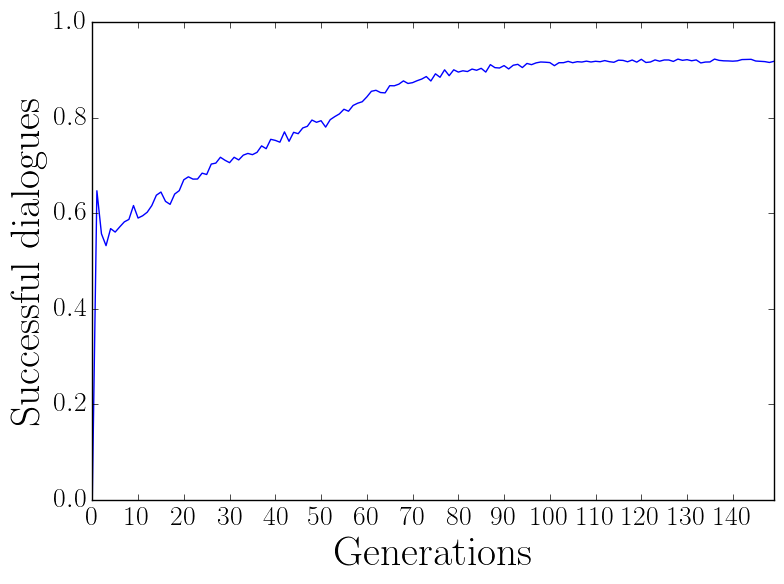
\includegraphics[width=0.49\linewidth]{fig/Results/Exp6/SuccDialogues1}\label{fig:succDia6}}
    \par \bigskip
    \subfigure[]{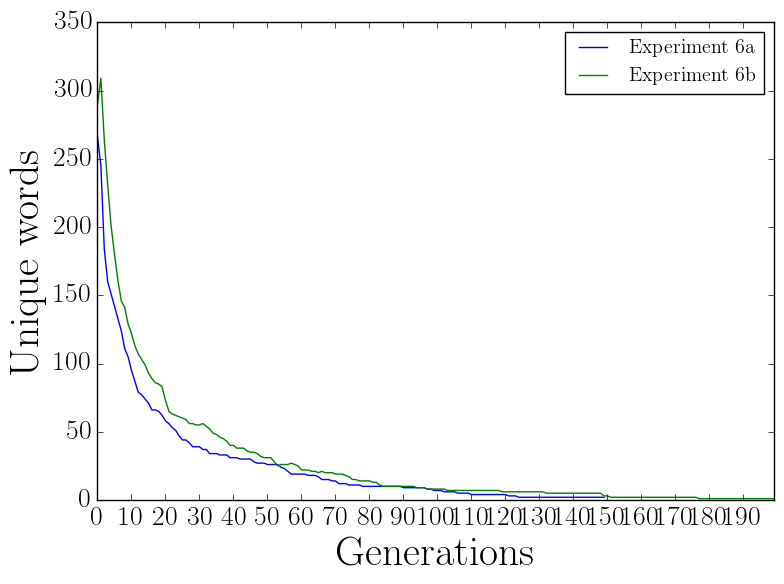
\includegraphics[width=0.6\linewidth]{fig/Results/Exp6/UniqueWordsAB}\label{fig:uniqueWords6}}
    \caption{Results from experiment 6. \subref{fig:Vocabulary6}: average vocabulary size of experiment 6a. \subref{fig:succDia6}: successful dialogues divided by total number of dialogues of experiment 6a. \subref{fig:uniqueWords6}: the number of unique highest ranked words in the population of experiment 6 a and b.}
    \label{fig:exp6.1}
\end{figure}

\clearpage
\subsection{Experiment 7 - making up new words}
Experiment 7 was conducted in two parts, both with an added probability for agents to invent a new word even though they had at least one word in their vocabulary. See Figures~\ref{fig:exp7.0} and \ref{fig:exp7.1} for the results from the two parts of the experiment.

Experiment 7a was performed with the probability of inventing a new word set to $25\%$. The average fitness stabilised at $0.37$, and the average degree stabilised at about $6.5$, as seen in Figures~\ref{fig:Fitness7} and \ref{fig:Degree7}. Both of these values were considerably lower than in experiment $1$. Figures~\ref{fig:Vocabulary7} and \ref{fig:succDia7} show that average vocabulary size was $6$ and the percentage of successful dialogues quickly reached $0.5$ but it did not slowly increase like in the previous experiments. The number of unique highest ranked words evolved similarly to experiment $1$, as seen in Figure~\ref{fig:uniqueWords7}. The population reached consensus at generation $68$, only six generations experiment $1$. 

Experiment 7b was performed with the probability of inventing a word increased to $45\%$. See figure~\ref{fig:uniqueWords7} for the figure related to this experiment. The other graphs have not been included because the purpose of this experiment was to see how the evolution towards consensus changed with a higher probability of inventing a word. The number of unique words quickly dropped to about five, but from five it struggled to actually reach consensus. Experiment 7b reached consensus at generation $73$, but that only lasted a few generations. For the remainder of the simulation, the number of unique words varied from one to four. 

\begin{figure}[htbp]
    \centering
    \subfigure[]{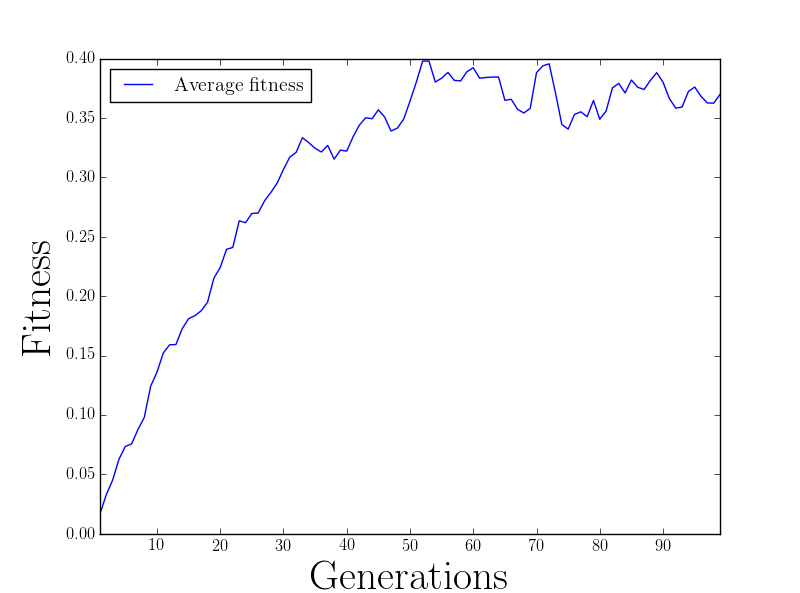
\includegraphics[width=0.49\linewidth]{fig/Results/Exp7/Fitness1}\label{fig:Fitness7}}
    \hfill
    \subfigure[]{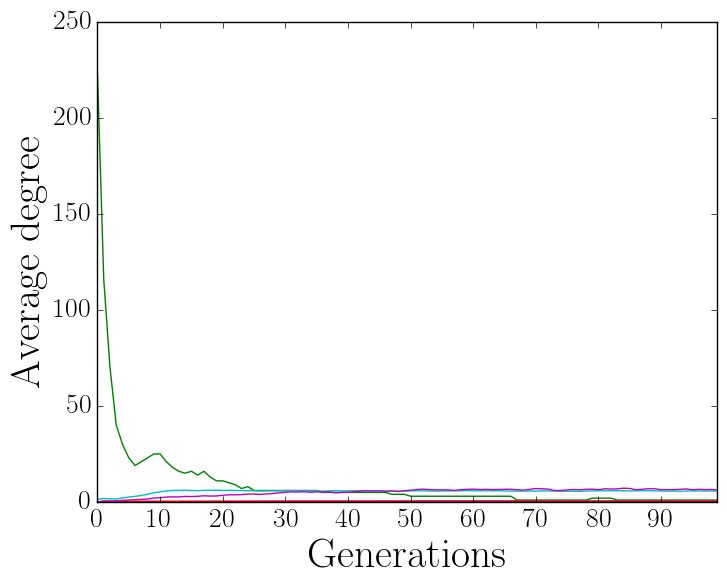
\includegraphics[width=0.49\linewidth]{fig/Results/Exp7/Degree1}\label{fig:Degree7}}
    \caption{Graphs from experiment 7.}
    \label{fig:exp7.0}
\end{figure}
\begin{figure}
    \centering
    \ContinuedFloat
    \subfigure[]{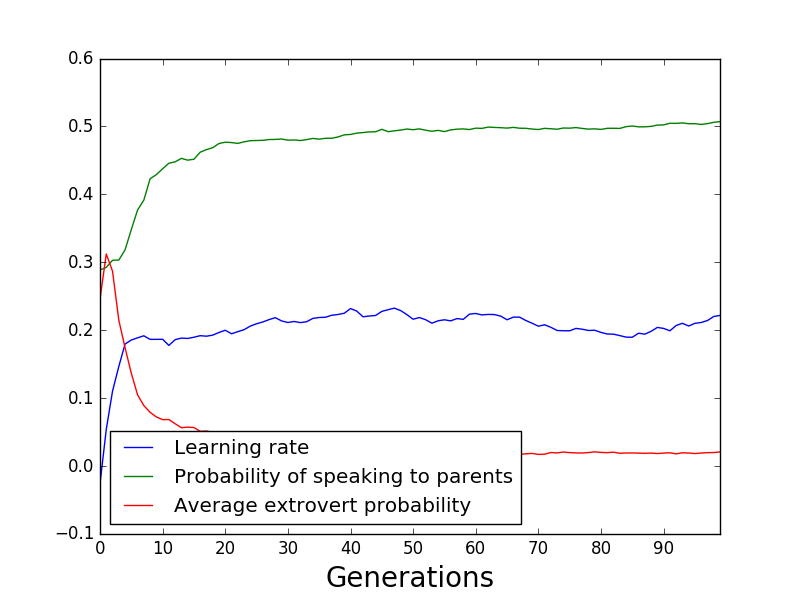
\includegraphics[width=0.49\linewidth]{fig/Results/Exp7/Genes1}\label{fig:Genes7}}
    \hfill
    \subfigure[]{\includegraphics[width=0.49\linewidth]{fig/Results/Exp7/Vocabulary1}\label{fig:Vocabulary7}}
    \par \bigskip
    \subfigure[]{\includegraphics[width=0.49\linewidth]{fig/Results/Exp7/SuccDialogues1}\label{fig:succDia7}}
    \hfill
    \subfigure[]{\includegraphics[width=0.49\linewidth]{fig/Results/Exp7/UniqueWordsAB}\label{fig:uniqueWords7}}
    \caption{Results from experiment 7. \subref{fig:Genes7}: the evolution of the traits from the genome. The three graphs in the figure are the green graph which is the average probability of conducting parent-child dialogues, the blue graph which is the average learning rate, and the  red graph which is the average probability of acting extrovertly. \subref{fig:Vocabulary6}: average vocabulary size of experiment 7a. \subref{fig:succDia6}: successful dialogues divided by total number of dialogues of experiment 7a. \subref{fig:uniqueWords6}: the number of unique highest ranked words in the population of experiment 7a and b.}
    \label{fig:exp7.1}
\end{figure}